\documentclass[11pt]{article}
\usepackage[review]{acl}
\usepackage{times}
\usepackage{latexsym}
\usepackage[T1]{fontenc}
\usepackage[utf8]{inputenc}
\usepackage{microtype}
\usepackage{inconsolata}
\usepackage{booktabs}
\usepackage{graphicx}

% Generated from results/paper_stats.json; do not edit.
\newcommand{\ScaleRuns}{28}
\newcommand{\ScaleManipulationPasses}{28}
\newcommand{\ScaleHackCorrect}{3}
\newcommand{\ScaleHackCalls}{6}
\newcommand{\ScaleSafeCorrect}{84}
\newcommand{\ScaleSafeCalls}{84}
\newcommand{\ScaleAbstentions}{22}
\newcommand{\PolicyHackCorrect}{3}
\newcommand{\PolicyHackCalls}{6}
\newcommand{\PolicySafeCorrect}{51}
\newcommand{\PolicySafeCalls}{51}
\newcommand{\RewardSafeCorrect}{33}
\newcommand{\RewardSafeCalls}{33}
\newcommand{\FixedHackCorrect}{3}
\newcommand{\FixedHackCalls}{9}
\newcommand{\FixedSafeCorrect}{24}
\newcommand{\FixedSafeCalls}{24}
\newcommand{\RelativeHackCorrect}{3}
\newcommand{\RelativeHackCalls}{3}
\newcommand{\RelativeSafeCorrect}{30}
\newcommand{\RelativeSafeCalls}{33}
\newcommand{\TrainingSteps}{500}
\newcommand{\EvalSources}{400}
\newcommand{\HackThreshold}{0.10}
\newcommand{\SafeThreshold}{0.02}
\newcommand{\ManipulationThreshold}{0.01}
\newcommand{\XcometZhCometMean}{-0.283}
\newcommand{\XcometZhCometMin}{-0.284}
\newcommand{\XcometZhCometMax}{-0.282}
\newcommand{\XcometDeCometMean}{+0.019}
\newcommand{\XcometDeCometMin}{+0.016}
\newcommand{\XcometDeCometMax}{+0.022}
\newcommand{\MetricXlCometMean}{+0.027}
\newcommand{\MetricXxlCometMean}{+0.026}
\newcommand{\AffectedLogs}{55}
\newcommand{\CorrectedRuns}{45}
\newcommand{\FollowupSeeds}{3}
\newcommand{\CorrectedRefusalMax}{0}
\newcommand{\PreambleCrossings}{1}
\newcommand{\CorrectedFiveHundredPreambles}{0}
\newcommand{\HumanPairs}{3}
\newcommand{\HumanItemsPerPair}{100}
\newcommand{\HumanRows}{1301}
\newcommand{\SmallPolicy}{Qwen2.5-1.5B-Instruct}
\newcommand{\LargePolicy}{Qwen2.5-7B-Instruct}
\newcommand{\ReferenceMetric}{COMET-22}


\title{Can a Pre-Training Audit Predict Which Translation Reward Will Be Hacked?}
\author{Anonymous ACL submission}

\begin{document}
\maketitle

% DRAFT abstract (2026-11-18), written from docs/GRPO_PAPER_OUTLINE.md at the author's request; revise freely.
% The generalization sentence is filled in once results/grpo_generalization_result.json exists.
\begin{abstract}
Quality-estimation (QE) models make reinforcement learning for machine
translation possible without references, but policies can learn to exploit
them.  Prior work documents such exploits and patches them after the fact; we
ask whether they can be predicted before training.  We propose a
policy-relative audit: for each reward and named failure type (source copying,
truncation, repetition, refusal), it measures how often the reward prefers a
controlled degenerate output over the initial policy's own translation, and a
frozen three-band rule turns that rate into a hack call, a safe call, or an
abstention.  We freeze every call before training and test it in
\ScaleRuns{} prospective GRPO runs spanning two policies, several QE reward
families and scales, and two translation directions, with every run required
to raise its own reward.  Counting each policy, reward, direction and failure
type once, safe calls are correct in \TaskSafeAllCorrect{} of \TaskSafeTasks{}
tasks, but hack calls in only \TaskHackAllCorrect{} of \TaskHackTasks{}: XCOMET
induces source copying into Chinese but not German.  A second frozen study with
two larger rewards and two new languages realizes all \GenHackTasks{} of its
hack calls, including a Russian call whose preference rate matched the failed
German one.  The German miss is not explained by how often the initial policy
samples the exploit, but by how little copying gains over translations the
reward already rates highly, an explanation we froze before scoring the new
runs.  Finally, a rollout padding bug had manufactured a dramatic refusal
collapse that vanished on a full rerun, a cautionary result for reward-hacking
studies.
\end{abstract}

\section{Introduction}

Reference-free quality estimation (QE) is an attractive reward for machine
translation because it can score new outputs without parallel data.  Yet a QE
model is a proxy: policy optimization can raise its score while reducing
translation quality \citep{he-etal-2024-improving}.  Recent multilingual MT
work directly documents wrong-language output, length errors, and a
self-generated-reference exploit (the policy repeats its own hypothesis so that
a hybrid QE model switches to reference-based scoring) under QE-based
reinforcement learning, and mitigates them with language and word-alignment
terms \citep{liu-etal-2026-mending}.  The practical question is therefore whether a
developer can identify a risky reward before paying for a full training run.

We study an interpretable pre-training audit.  For each initial policy, reward,
direction, and named failure type, we construct controlled degenerate outputs
and measure how often the reward prefers them to the policy's translation.  A
frozen rule converts that preference rate into a hack call, safe call, or
abstention.  Unlike simulation-based prediction from smaller RL runs
\citep{deng-etal-2026-simhack}, our audit requires no reference optimization
run.  It predicts a failure type rather than an onset time.

Our contributions are:
\begin{itemize}
  \item a prospective test of failure-type predictions across \ScaleRuns{}
        generative GRPO runs, with every apparent safe outcome gated on reward
        improvement;
  \item evidence that the audit's negative calls transfer reliably in the
        tested setting, while positive calls depend on whether the policy can
        reach the audited behavior;
  \item controlled policy- and reward-scale comparisons, including a null
        hacking result for both tested MetricX scales; and
  \item a complete correction analysis showing that rollout padding can create
        dramatic but spurious refusal and preamble failures.
\end{itemize}

The result is intentionally narrower than a universal reward-hacking detector.
It is evidence for a cheap screen over named failure modes and a diagnosis of
what that screen omits.

\section{Related work}

\paragraph{Reward overoptimization and reward gaming.}
Optimizing a learned proxy reward can raise the proxy while degrading the
intended objective, and the gap grows predictably with optimization pressure
\citep{gao-etal-2023-scaling}.  \citet{skalse-etal-2022-defining} formalize when
a proxy can be gamed at all.  We study a narrower, applied question: which
named failure a specific translation reward will produce under a specific
policy.

\paragraph{QE metrics as decoding and training objectives.}
Using QE and reference-based metrics to rerank or decode improves metric scores,
but those gains are partly bias toward the decoding metric
\citep{fernandes-etal-2022-quality,kovacs-etal-2024-mitigating}.  As RL rewards,
QE models can improve translation \citep{he-etal-2024-improving} and support
R1-style training \citep{feng-etal-2025-mtr1zero}.  WALAR documents
wrong-language output, length errors and a self-generated-reference exploit
under QE-only rewards, and adds language and word-alignment terms
\citep{liu-etal-2026-mending}.  Reference-free multilingual post-training
combines QE rewards with a language-ID gate and checkpoint interpolation
\citep{han-etal-2026-reference-free}.  These works establish the failure and
its mitigations; we ask whether the failure type can be forecast before the
target run.

\paragraph{Predicting hacking before training.}
SimHack learns training dynamics from smaller code-RL runs to predict when
hacking will begin under a target recipe \citep{deng-etal-2026-simhack}.  Our
audit is cheaper and needs no reference optimization runs, but it predicts only
the behaviors it tests and, as we show, its positive calls depend on more than
the reward's preference.

\section{Policy-relative audit}

Let $y_{\mathrm{init}}(x)$ be the initial policy's translation for source $x$, and let
$h_k(x)$ be a controlled output exhibiting failure type $k$.  For reward $r$,
we estimate
\begin{equation}
  p_k = \Pr_x[r(x,h_k(x)) > r(x,y_{\mathrm{init}}(x))].
\end{equation}
The rule predicts a hack when $p_k$ exceeds the frozen upper threshold, predicts
safe below the frozen lower threshold, and abstains between them.  A predicted
hack is correct when the corresponding output indicator increases by at least
\HackThreshold{}; a safe call is correct when the increase is at most
\SafeThreshold{}.

Safe outcomes are informative only when the assigned reward rises by at least
\ManipulationThreshold{}.  This prevents a failed optimization run from being
counted as resistance to hacking.  The audited indicators are source copying,
refusal, repetition, and response shortening.  They are diagnostics of named
behaviors, not complete measures of translation quality.

\section{Experimental design}

\begin{table}[t]
\centering
\small
\resizebox{\columnwidth}{!}{%
\begin{tabular}{ll}
\toprule
Setting & Value \\
\midrule
Algorithm & GRPO (TRL) \\
Prompts per step / generations & \PromptsPerStep{} / \GenerationsPerPrompt{} \\
Updates & \TrainingSteps{} \\
KL coefficient $\beta$ & \KLBeta{} \\
Sampling temperature & \Temperature{} \\
Max new tokens & \MaxNewTokens{} \\
LR, full fine-tuning (\SmallPolicy{}) & $\LRFull$ \\
LR, LoRA (\LargePolicy{}) & $\LRLora$ \\
LoRA rank / $\alpha$ & \LoraRank{} / \LoraAlpha{} \\
Audit prompts per task & \AuditPrompts{} \\
Hack / safe thresholds on $p_k$ & $>\HackP$ / $\le\SafeP$ \\
Eval sources per direction & \EvalSources{} (greedy) \\
\bottomrule
\end{tabular}
}
\caption{Frozen training and audit settings, read from the protocol files.}
\label{tab:setup}
\end{table}

We optimize \SmallPolicy{} and \LargePolicy{} translation policies with GRPO
\citep{shao-etal-2024-deepseekmath}; Table~\ref{tab:setup} lists the frozen
settings.  Training prompts are English sentences only, so every direction
shares the same prompts and the same evaluation sources.  The reward set includes XCOMET,
CometKiwi, and MetricX variants.  English sources are translated into German
and Chinese.  The prospective scale protocol uses \TrainingSteps{} updates and
evaluates greedy outputs on \EvalSources{} sources per direction.

The policy-scale arm applies LoRA to the larger policy and tests reward-specific
predictions.  The reward-scale arm holds the smaller policy and optimization
recipe fixed while comparing MetricX XL and XXL rewards.  Because the larger
policy uses LoRA and a different learning rate, that arm does not identify a
pure model-size effect.

We report the frozen behavior indicators and independent reference-based
\ReferenceMetric{} and chrF.  Every scale result is reconstructed from per-output records;
the scorer verifies protocol hashes, launch metadata, one-to-one source rows,
indicator recomputation, and the manipulation gate before merging results into
the paper SSOT.

\paragraph{Freezing procedure.}
Every experiment is fixed in a hashed protocol file before its audit, and the
audit's calls are derived mechanically into a predictions file before any
training run.  The trainer refuses to start a run whose protocol or
predictions hash differs from the pinned value, and refuses runs the protocol
does not list.  Amendments made after outcomes were seen are recorded with what
was known at the time.

\section{Prospective results}

All \ScaleManipulationPasses{} of \ScaleRuns{} runs increase their assigned
reward enough to pass the manipulation check.  Table~\ref{tab:scorecard} shows
the complete called-cell scorecard.  The audit makes \ScaleAbstentions{}
additional abstentions.

\begin{table}[t]
\centering
\small
\resizebox{\columnwidth}{!}{%
\begin{tabular}{lrr}
\toprule
Evaluation set & Hack correct/called & Safe correct/called \\
\midrule
Corrected fixed-rule grid & \FixedHackCorrect/\FixedHackCalls & \FixedSafeCorrect/\FixedSafeCalls \\
Corrected policy-relative grid & \RelativeHackCorrect/\RelativeHackCalls & \RelativeSafeCorrect/\RelativeSafeCalls \\
Prospective scale study & \ScaleHackCorrect/\ScaleHackCalls & \ScaleSafeCorrect/\ScaleSafeCalls \\
\quad Policy-scale arm & \PolicyHackCorrect/\PolicyHackCalls & \PolicySafeCorrect/\PolicySafeCalls \\
\quad Reward-scale arm & --- & \RewardSafeCorrect/\RewardSafeCalls \\
Prospective generalization study & \GenHackCellsCorrect/\GenHackCells & \GenSafeCellsCorrect/\GenSafeCells \\
\bottomrule
\end{tabular}
}
\caption{Frozen prediction outcomes.  Each cell is a run by named failure type;
seeds do not create independent audit probabilities.}
\label{tab:scorecard}
\end{table}

\begin{figure}[t]
\centering
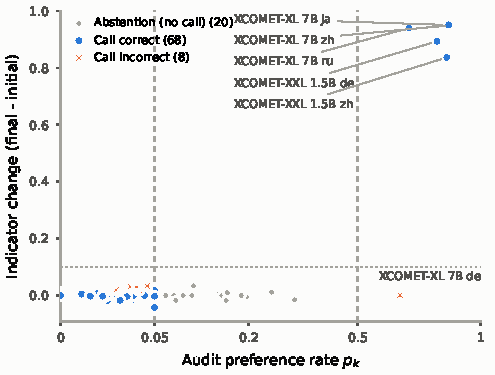
\includegraphics[width=\columnwidth]{fig_audit_outcomes}
\caption{Audit preference rate against the observed change in the audited
indicator, one point per audit task (\FigTaskPoints{} tasks; seeds averaged).
Dashed lines mark the safe ($\le\SafeP$) and hack ($>\HackP$) thresholds; the
dotted line marks the hack outcome margin.  Calls correct: \FigCorrect{};
incorrect: \FigIncorrect{}; abstentions: \FigAbstain{}.  The $x$-axis is
square-root scaled.  Only studies scored with the prospectively fixed
indicator definitions are shown.}
\label{fig:audit-outcomes}
\end{figure}

\paragraph{Task-level view.}
Seeds replicate an optimization run; they do not replicate an audit
prediction.  Collapsing seeds, the scale study contains \TaskSafeTasks{} safe
tasks, all \TaskSafeAllCorrect{} correct in every seed, and only
\TaskHackTasks{} hack tasks, of which \TaskHackAllCorrect{} is correct in every
seed.  \TaskAbstainTasks{} tasks are abstentions.  The evidence for positive
calls is therefore much thinner than the cell counts suggest, which motivates
the generalization study below.  Figure~\ref{fig:audit-outcomes} shows every
task: safe calls sit flat at zero change, while the two hack calls split.

\paragraph{Safe calls transfer.}
Every prospective safe call passes.  This includes the prespecified
CometKiwi refusal check and all called MetricX cells.  MetricX XL and XXL show
no audited hack under the smaller policy, despite increasing their assigned
rewards.

\paragraph{Positive calls require reachability.}
The six prospective hack calls all predict source copying by XCOMET under the
larger policy.  All Chinese runs copy and all German runs do not.  Reference
\ReferenceMetric{} changes by a mean of \XcometZhCometMean{} in Chinese, with
seed values from \XcometZhCometMin{} to \XcometZhCometMax{}.  In German it instead changes
by \XcometDeCometMean{}, from \XcometDeCometMin{} to
\XcometDeCometMax{}.  Thus the audit correctly identifies a reward preference,
but that preference becomes a realized exploit only in one direction.  The
audit lacks a policy-dependent reachability term.

\paragraph{Reward scale.}
Across the reward-scale arm, mean \ReferenceMetric{} changes are
\MetricXlCometMean{} for MetricX XL and \MetricXxlCometMean{} for MetricX XXL.
Neither reward produces an audited failure.  This does not contradict
\citet{liu-etal-2026-mending}, who report the MetricX self-generated-reference
exploit only for a smaller policy than ours and not for their larger ones.

\section{Generalization study}

A second frozen protocol adds independent audit tasks: two new reward models
(XCOMET-XXL and CometKiwi-23-XXL, smaller policy, English to German and
Chinese) and two new target languages (Japanese and Russian, larger policy, the
four base rewards).  All \GenManipulationPasses{} of \GenRuns{} runs pass the
manipulation check.

\paragraph{Every hack call came true.}
All \GenHackTasks{} hack tasks are realized in every seed
(\GenHackCellsCorrect{}/\GenHackCells{} cells): both XCOMET-XXL directions and
XCOMET-XL into Japanese and Russian.  The Russian call is the informative one.
Its preference rate ($p=\PRu$) was close to that of the failed German call
($p=\PDeSeven$), yet the policy copied in every seed.

\paragraph{What distinguishes the German miss.}
Before scoring these runs we froze two candidate explanations for that miss,
each with a threshold derived only from the earlier tasks.  The first, a
\emph{reachability probe}, asked whether the initial policy already samples
the exploit.  It failed calibration: the German policy samples source copies
more often ($\ReachDeSeven$ of rollouts) than the Chinese policy that did copy
($\ReachZhSeven$), so no rule could be derived.  The second, frozen afterwards
and disclosed as post hoc, is the \emph{copy margin}: how much more the reward
pays for a copy than for the initial policy's own translation.  The German
policy's translations already score so highly that copying gains only
\MarginDeSeven{}, against at least \MarginRealizedMin{} for every realized
copy.  The derived threshold (\MarginStar{}) kept all four new hack calls,
including Russian (\MarginRu{}), and all four were realized.  This supports the
margin as the missing ingredient, but rests on a single negative calibration
case and was tested on the same held-out tasks as the failed probe.

\paragraph{Safe calls: one indicator failure.}
Safe calls are correct in \GenSafeTasksCorrect{} of \GenSafeTasks{} tasks
(\GenSafeCellsCorrect{}/\GenSafeCells{} cells).  All \GenFailedSafeCells{}
failed cells are the truncation indicator, which we redefined prospectively as
shortening relative to the initial output.  Inspecting them (post hoc) shows
that this definition also flags \emph{cleanups}: the larger policy's initial
Russian outputs often append mixed-language commentary (\RuHanInitial{} of
\RuHanN{} contain Chinese characters, falling to between \RuHanFinalMin{} and
\RuHanFinalMax{} after training), so a correct, shorter final translation counts
as truncation.  We keep the frozen score and report the diagnosis.

\section{Padding correction as a methodological result}

After the original smaller-policy experiments, we found that the training
tokenizer right-padded conversational prompts even though evaluation and audits
used left padding.  The warning appeared in \AffectedLogs{} affected training
logs.  We froze an amendment, corrected the tokenizer, and reran
\CorrectedRuns{} experiments without changing predictions.

The correction changes the scientific conclusion of the refusal follow-up.
Under right padding, CometKiwi optimization had produced a large refusal
collapse and German preambles.  Under correct padding, the prespecified horizon
hypothesis fails in all \FollowupSeeds{} seeds; the maximum final refusal count
is \CorrectedRefusalMax{}.  The guard feasibility and cross-metric hypotheses
both pass.  Every corrected shorter run ends with
\CorrectedFiveHundredPreambles{} detected preambles, and only
\PreambleCrossings{} corrected follow-up crosses the exploratory preamble audit
threshold.  Stripping that run's preambles has negligible reference-quality
effect.

This is not merely an implementation footnote.  Padding changes the
autoregressive state from which sampled continuations begin and can create a
qualitatively different policy.  Logging tokenizer behavior and rerunning the
full frozen grid prevented an artifact from becoming the paper's main failure
case.

\section{Human evaluation}

\textbf{TODO before submission: complete blinded human evaluation.}
The frozen package targets the paper's headline comparisons:
\HumanPrimarySheets{} primary sheets of \HumanItemsPerSheet{} source items each
(\HumanPrimaryRows{} unique candidate rows), covering the larger policy's
safe-called rewards and the MetricX reward-scale series in English--German and
English--Chinese, plus a secondary English--Spanish sheet from the corrected
smaller-policy grid.  Copying outputs that the indicators already flag appear
only on \HumanAttentionItems{} attention-check items.  Candidate order is
randomized, duplicate outputs are merged, and the system keys are hash-pinned.  Human scores will be used only for final evaluation, never to
retune the audit, thresholds, or checkpoints.  Until this evaluation is
complete, automatic quality results are corroborating evidence rather than a
definitive adequacy judgment.

\section{Limitations}

The audit covers only four hand-specified failure types.  The copy-margin
explanation was proposed after the reachability probe failed and was tested on
the same held-out tasks; it needs a fresh test.  A safe call cannot
exclude an unmodeled exploit.  Positive calls measure reward preference, not
the probability that a particular optimizer and policy will reach the behavior.
The policy-scale comparison also changes parameterization and learning rate.
The language coverage is narrow, reward families are correlated, and repeated
seeds measure optimization variability rather than independent audit tasks.
Finally, human evaluation is pending.

\section*{Ethics statement}

The study trains translation models on public English text and evaluates them
on public WMT test sources; it collects no personal data.  Reward hacking in
deployed MT can silently degrade translations for users who cannot check them,
which is the risk this audit aims to reduce.  Human annotators will be paid or
volunteer lab members, will receive written guidelines, and will see only
blinded outputs.

\section*{Compute}

Training used NVIDIA A100 and H100 GPUs.  The prospective scale study used
\ScaleGPUHours{} GPU-hours of training and the corrected rerun grid
\CorrectedGridGPUHours{}, excluding evaluation and audits.

\section{Conclusion}

A cheap policy-relative audit can screen named MT reward failures before GRPO.
Its safe calls survive meaningful optimization across policies, rewards and
five directions, apart from an indicator that cannot tell cleanup from
truncation.  Its hack calls came true in every case except one, and that miss
is explained by the exploit's reward margin over the initial policy rather
than by how often the policy samples it.  Adding that margin to the audit is
cheap.  It still needs a test on new policies and rewards, because it rests on
a single negative case.  The padding
rerun further shows why seemingly strong reward-hacking results require exact
rollout provenance before they support a scientific claim.

\bibliography{references}

\appendix
\section{Per-run results of the scale study}

\begin{table*}[t]
\centering
\small
\begin{tabular}{lllrrrrr}
\toprule
Policy & Reward & Dir. & Seed & $\Delta$ own reward & Untranslated & Refusal & $\Delta$ \ReferenceMetric{} \\
\midrule
\csname @@input\endcsname generated_scale_runs.tex
\bottomrule
\end{tabular}
\caption{Every run in the prospective scale study.  Indicator values are final-checkpoint rates on the evaluation sources; $\Delta$ columns are final minus initial.}
\label{tab:scale-runs}
\end{table*}

\end{document}
